\documentclass[11pt]{article}
%\usepackage{abbrevs}
\usepackage{natbib}
\usepackage{hyperref}
\usepackage{graphicx}     % could insert ``draft'' between []
\usepackage{caption}
\usepackage{subcaption}
\pagestyle{empty}

\setlength{\oddsidemargin}{0pt} % there is 1 inch before the
                                % side margin in ``article'' class
\setlength{\textwidth}{6.5in}

\setlength{\voffset}{0pt}
%\setlength{\topmargin}{-36pt}     % there is 1 inch before the
\setlength{\topmargin}{-0.75in}     % there is 1 inch before the
                                % top margin in ``article'' class and
                                % then room for header, etc.
\setlength{\textheight}{9.5in}
%%%%%%%%%%%

\begin{document}
{\centering{\bf\Large HERA:  Discussion Design} \\}
{
\centering{\bf\large Hydrogen Epoch of Reionization Array \\}
}
\vspace*{0.5cm}

%\tableofcontents
%\newpage

\section{Introduction}

The Hydrogen Epoch of Reionization Array (HERA) project 

This document provide an initial discussion design (aka strawman).  It is meant
to introduce one plausible system design for discussion.  The design is then to
be iterated to the point of a first version of a real architecture and design.
Figure \ref{fig:overall} shows an overall block diagram of the system,
identifying the major subsystems, which are discussed below.  Note that blocks
bordered with dashed lines indicate optional or variational elements.

The design is for about 1000 elements.  As discussed below, the elements will
likely be aggregated in groups of three at the node and groups of eight in the
digital system, so the target number is 3 $\times$ 8 $\times$ 42 = 1008
elements.

\begin{figure}[h]
\centering
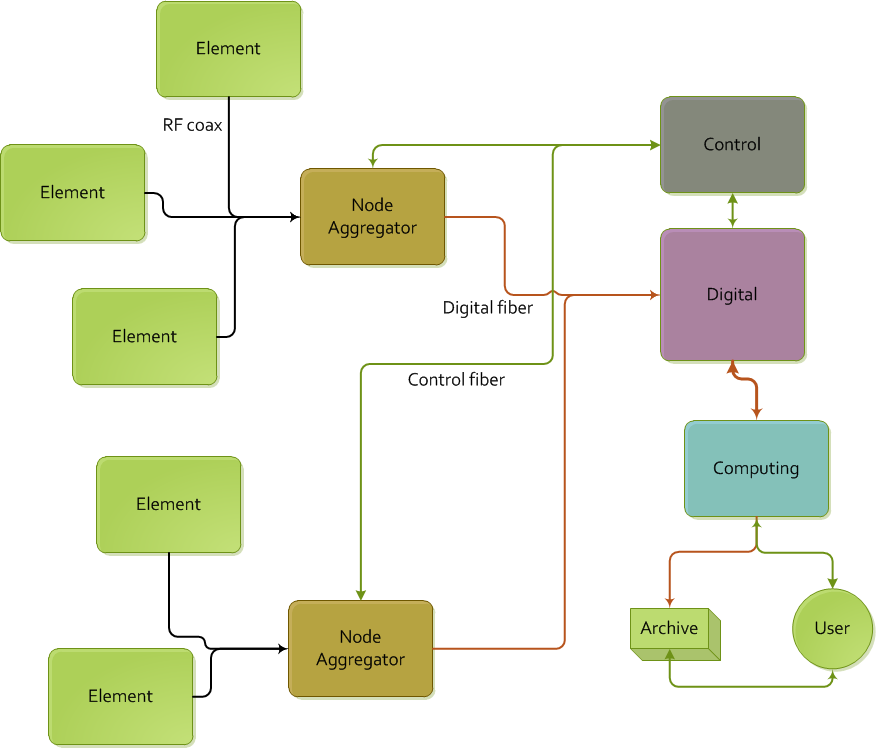
\includegraphics[width=0.75\textwidth]{plots/Overall.png}
\caption{Overall system block diagram.}
\label{fig:overall}
\end{figure}

\section{Feed}
\label{sec:feed}

\begin{figure}
\centering
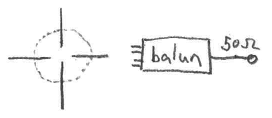
\includegraphics[width=3in]{plots/feed.png}
\caption{Antenna feed, with active balun.  Output is $50\Omega$ coaxial cable for two polarizations.}
\label{fig:feed}
\end{figure}

Desirable features of the antenna feed are:
\begin{itemize}
\item bandwidth $\sim$1 octave (100-200 MHz)
\item evolution of gain versus frequency $\ll$ frequency structure intrinsic to foregrounds
\item stability of gain versus time and temperature
\item matching of polarization beams to minimize polarization leakage
\item first-stage amplification with $T_{\rm LNA}\ll T_{sky}$. Of order 100 K.
\end{itemize}

We currently have two feeds that have been field-tested: the PAPER feed and the MWA feed (of which
16 make up an MWA title).  Both designs use linear polarization feeds.  These are relatively
straight-forward to make, but tend to have significant problems with polarization leakage
over wide fields of view.

ISSUES: need for resistor load and/or phase switch at feed?

\subsection{PAPER Feed}

The PAPER feed is a dual-polarization approximation to a sleeved dipole design that approximately matched
to a 100-200 MHz bandwidth.  The PAPER feed's frequency evolution, when paired with a flapped groundscreen
that approximates a corner reflector (\S\ref{sec:element}), has been demonstrated to have many of the properties
necessary for the delay-spectrum approach to foreground avoidance.  PAPER feeds are currently relatively expensive
per item, and could benefit from an iteration of design for manufacture.

Although PAPER does reasonably well with $75\Omega$ coaxial cable connecting antenna feeds to receivers,
the necessary transition from $75\Omega$ to the $50\Omega$ SMA standard used within the correlator requires
an impedance matching network that can easily cause problematic signal reflections.  We suggest that it
would be better to push the impedance mismatch up to the very front of the system.

%\begin{table}[h]
%\begin{center}
%\caption{\label{tab:feed}Antenna Feed Costing}
%\begin{tabular}{ | p{2in} | c | c | r |}
%\hline
%\bf Description & \bf Each & \bf Number & \bf Total [k] \\
%\hline
%Dipole & \$50 & 1008 & \$50 \\
%Balun & \$250 & 1008 & \$250 \\
%Labor & \$100 & 1008 & \$100 \\
%\hline
%\end{tabular}
%\end{center}
%\end{table}

\subsection{MWA Feed}

The MWA feed follows a bowtie design that has a substantially wider operational bandwidth (XXX--300 MHz) 
than PAPER feeds.  It has not yet been demonstrated whether these feeds have the properties necessary
for delay-spectrum foreground avoidance.  MWA elements have undergone a design for manufacture step, and
are relatively inexpensive per item.  In particular MWA LNAs are much cheaper (by an order of magnitude)
than PAPER baluns.

Has there been any significant study of single MWA feeds (i.e. not part of a beamformed tile)?

%It would be nice to add the MWA feed costing as another data point.

\section{Element}
\label{sec:element}

The element sub-system is meant to maximize the sensitivity with minimal
hardware.  The design of the element, which integrates a feed
(\S\ref{sec:feed}) with a reflective structure, is central to both the
foreground response of the instrument, and the overall sensitivity.

There is much that we still do not know about the problem of suppressing
foregrounds to the 21cm signal from the Epoch of Reionization.  Many approaches
have been proposed, but without a detection, it is hard to know which approach
will ultimately be the most successful.  However, there is some convergence
around the idea of the foreground ``wedge'' that represents a baseline-length
dependent threshold for where smooth-spectrum foreground emission can enter an
interferometric measurement.  Experiments then have a choice of whether to
pursue a detection of 21cm EoR emission within the wedge, which requires yet
undemonstrated levels of calibration and foreground modeling, or to work
outside of the wedge and shoulder more stringent sensitivity requirements.

There are limits to this characterization.  Models of the 21cm EoR power
spectrum tend to fall off below $k\sim 0.1h {\rm Mpc}^{-1}$, indicating that
the sensitivity benefits of working at smaller $k$ do not hold indefinitely.
Moreover, there are foregrounds/systematics that arise outside of the wedge
(with polarization leakage being most likely the worst) that require a strategy
even for experiments working outside of the wedge.

With polarization leakage being one of the biggest concerns
that has yet to be addressed, it will be important to provide several pathways to
mitigate this potential issue.  One important pathway to doing this is in the design of the
element itself.  
The element
may restrict the field of view or otherwise compenste for differences in polarization beams
so as to mitigate polarization leakage issues.
The MWA and PAPER are just on the cusp of being able to study the polarization
leakage for these elements.  \citet{moore_et_al2013} predict that without direction-dependent
calibration, PAPER leakage will be $\sim$5\%, and depending on how polarized foregrounds
behave, this may cause a systematic bias in measured power spectra of around 1000 mK$^2$ between
$0.2\le k\le 1.0h {\rm Mpc}^{-1}$.  
One potential approach to mitigating raw polarization leakage is to design elements that do a better
job of matching polarization beams.  This might be done through apodization (at low frequencies, this
might even be done by overilluminating a reflector), or by tailoring a reflector to match beams.
PAPER is currently demonstrating how fringe-rate filters can be used to tailor beam responses between
declination bins.  This may be used to reduce a 2D beam matching problem to a 1D problem.

In general, we propose that HERA adopt a strategy of bringing enough sensitivity on shorter
baselines to avoid the necessity of working inside of the wedge for the key
EoR science goals, but to provide the ``hooks'' for the possibility of
eventually working within the wedge.  In essence, this entails designing
elements tailored to a delay-spectrum approach to detecting 21cm EoR, but
addressing the needs of imaging, etc., in the array configuration.
A key requirement for any element used in 21cm intensity mapping is that resonances and reflections
within the element not modulate otherwise spectrally-smooth foreground emission on frequency scales
that one might hope to measure the high-redshift 21cm signal.

Desirable features of elements (apart from feeds) are:
\begin{itemize}
\item ability to be placed within 30m (or better, 16m) of one another to support the
short baselines required by delay-spectrum foreground avoidance
\item reflections arising from foreground signals bouncing within the element
be attenuated by -60dB for time delays $\tau<100 {\rm ns}$
\item polarization beams matched to better than 0.5\%, or if this is not possible, matched
at this level following a reweighting along one axis (i.e. declination contours, as discussed above)
\item maximal collecting area (or rather, minimal beam area) given constraints above.  As shown
in Appendix B of \citet{parsons_et_al2013}, the key sensitivity metric here is 
$\Omega^\prime=\frac{\Omega_{\rm P}^2}{\Omega_{\rm PP}}$
\item ruggedness
\end{itemize}

We currently have three different designs on the table.  The PAPER element uses a reflective groundscreen
with flaps that approximates a corner reflector for a dipole feed.  The MWA element consists of 16
feeds closely packed on a reflective screen.  A third design is a parabolic dish approximately
10 m in diameter with a focal length of 3.5 m, statically pointing up.

ISSUES: is spec on polarization leakage attainable?  Tracking vs. drift-scanning.  Is the spec
on reflections attainable for an obstructed aperture such as a parabolic dish?

\subsection{PAPER Groundscreen}

PAPER groundscreens are currently one of the smallest elements being used for 21cm EoR analysis.
This comes at a significant penalty in sensitivity.  However, per feed, they nearly maximize
collecting area without obstructing the aperture, and have very little capacity for internal
reflection, which make them very effective for delay-spectrum analysis.  Polarization leakage
may be a significant problem for these elements, however.  They are great for wide-field imaging.

Estimated area: 8 m$^2$.  $\Omega^\prime=2.35 {\rm sr}$.

\subsection{MWA Tile}

This element concept is best exemplified by the MWA tile design.
For tile elements, we assume drift-scan observations using
static beamforming.  This choice is definitely debatable, but 
the thinking is that the enhanced sensitivity of multiple beams
may be outweighed by the associated complexity and cost of operation and calibration.

The sub-system consists of identical elements that are aggregated at
a node.  The connection between the two has the following interfaces:

\begin{itemize}
\item Two RF cables (50 $\Omega$, Type-N)
\item DC power (2-conductor \#18)
\item Ground (1-conductor \#18)
\item Control (2-conductor \#24)
\end{itemize}

Figure \ref{fig:elements} shows two possible layouts of dipoles as well as
indicating the accompanying RF hardware possibilities.  An optional phase
switch is shown, which may also go at the node or be omitted.  It is not
desired to have at the element since logic or faster switching signals are then
needed at that location, however it has the greatest potential performance at
that location.

\begin{figure}
\begin{subfigure}[h]{0.5\textwidth}
\centering
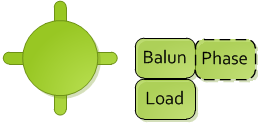
\includegraphics[width=\textwidth]{plots/Element1.png}
\caption{Single-dipole element.}
\label{fig:element1}
\end{subfigure}
\begin{subfigure}{0.5\textwidth}
\centering
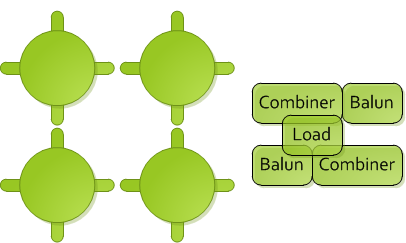
\includegraphics[width=\textwidth]{plots/Element4.png}
\caption{Four-dipole element.}
\label{fig:element4}
\end{subfigure}
\caption{Element configurations.}
\label{fig:elements}
\end{figure}

In order to maximize sensitivity for a given size correlator, the dipoles may
be combined in a static, zenith beamformer (combiner).  Depending on the
performance details, the combiner may precede the balun to limit hardware
needed.

Estimated area: 16 m$^2$.  $\Omega^\prime\approx0.18\ {\rm sr}$.

\subsubsection{Sparse Tiles}

The rationale here is that, although imaging requires that grating sidelobes be suppressed by
spacing feeds at $\lambda/2$ intervals, 21cm intensity mapping does not necessarily care.  In this
case, sub-elements with increased collecting area (think PAPER groundscreens) can be tiled at
intervals nearer to $\lambda$ in length, reducing the number of signal paths at the expense of
more infrastructure around each feed.  It turns out that the beam metric for tiles peaks
at $\lambda$ spacing.  Hence, if we modify the dense tile design above, it is possible to
get slightly improved performance.

Estimated collecting area: 22 m$^2$.
$\Omega^\prime\approx0.13\ {\rm sr}$.

\subsection{Parabolic Dish}

\begin{figure}
\centering
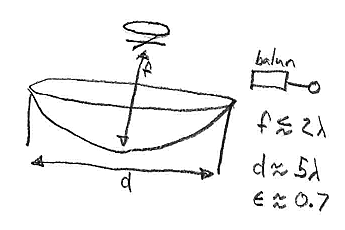
\includegraphics[width=3in]{plots/eor_dish.png}
\caption{}
\label{fig:element_dish}
\end{figure}

This element concept is novel, but bears similarities to a drift-scan observing mode explored on
the GMRT, and to the cylinder dish concept being explored for CHIME.  

In order for a parabolic (or cylindrical) dish to work for 21cm intensity mapping, the focal length
and dish diameter must be carefully controlled to avoid reflections that enter at a significant delay,
and thus modulate foregrounds to corrupt scales at the corresponding $k_\parallel$.  Based on recent work
characterizing foregrounds, it seems reasonable to ask that a dish not create more spectral structure than
the shortest ($8\lambda\approx15$m) baselines that have been shown to be well-behaved.  Beyond limiting
the dish diameter to 15m, this requirement restricts the focal length, since once of the primary resonances
in the dish will be the ``narcissistic waves'' that arise between the primary and secondary reflector and/or
the primary reflector and the antenna feed.  These latter waves are a consequence of the necessarily
imperfect match of the feed electronics to the impedance of free space.

To mitigate narcissistic refletions, one typically adds an attenuator or ``splash cone'' directly below the feed.
If we posit that reflections must be suppressed by $-60$dB at delays corresponding to the time it takes
to travel 15m, and if we assume that reflections are attenuated by a factor $A$ for each crossing of the
attenuator placed below the feed, then the number of allowed reflections, $R$, is given by
\begin{equation}
R={\rm floor}\left(\frac{-60{\rm dB}}{2A}\right).
\end{equation}
Thus, for a feed height (or focal length), $f$, we have
\begin{equation}
2Rf<15{\rm m}.
\end{equation}
For a moderate attenuation value of $A=-15$dB, we have $f<4$m.

\begin{figure}
\centering
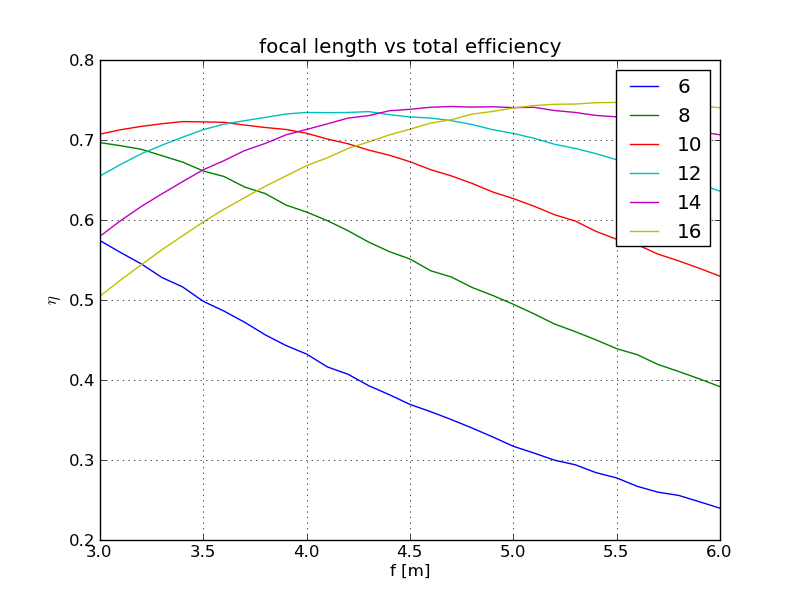
\includegraphics[width=4in]{plots/focal_len_vs_eff.png}
\caption{Total efficiency as a function of focal length, for various diameters of parabolic dishes (in meters).
Choosing a fiducial focal length of $f=3.5$m, dish diameters of $10\le d\le 12$m yield efficiencies of
$\eta\sim0.7$.}
\label{fig:focal_len_vs_eff}
\end{figure}

As shown in Figure \ref{fig:focal_len_vs_eff}, for a chosen focal length of $f=3.5$m, dish diameters in the
range of 10 to 12m yield efficiencies of $\epsilon\approx0.7$.  Hence, the total effective collecting area
of a dish that has been tuned for 21cm intensity mapping at EoR frequencies is of order $80{\rm m}^2$.  The
corresponding effective beam area at 150 MHz 
(noting the issue described in \S\ref{sec:beam_area}) is approximately
\begin{equation}
\Omega^\prime\approx0.06\ {\rm sr}.
\end{equation}

In addition to the substantial collecting area that this design provides, the relatively narrow field of
view associated with a larger dish may go a long way toward mitigating some of the polarization leakage
problems that are just on the horizon of being discovered with current designs.  However, without concrete
measurements, this is largely speculation.

\section{Node}

A node is responsible for receiving signals from 30 elements, providing secondary amplification,
digitizing each signal, and transmitting packetized data over an optical link to a central location
(see Figure \ref{fig:node}).  Nodes are evisioned to be small thermally controlled enclosures that host
receiver cards (providing filtering \& amplification of RF signals) and digitizers (sampling $\ge$6 RF signals,
corresponding to 2 dual-polarization antennas, outputting 10 GbE packetized data via SFP+ ports), along
with associated power supplies, cables, sensors, and control systems.  There will be 34 nodes in the system (for
1020 elements).

Desirable features in a node are:
\begin{itemize}
\item secondary amplification that is a negligible (< 10 K) source of thermal noise
\item thermal and electrical stability
\item 100 dB RFI shielding
\item better than -40 dB shielding between signal paths
\end{itemize}

\begin{figure}[h]
\centering
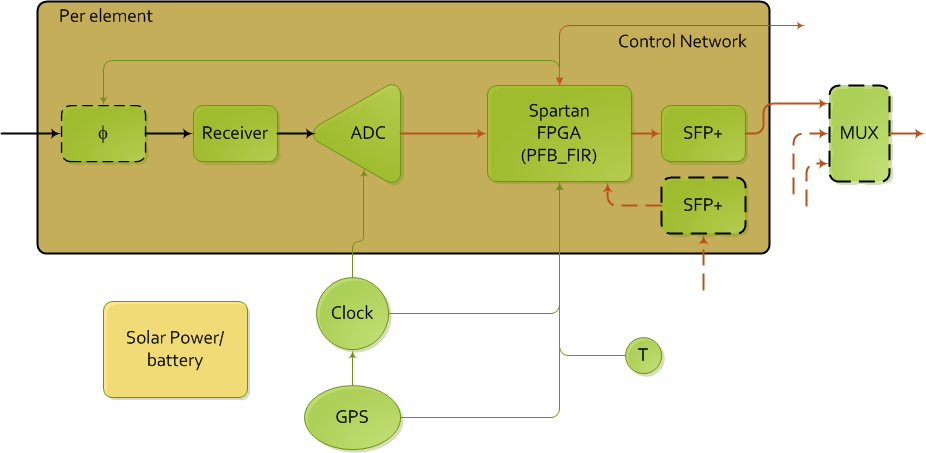
\includegraphics[width=0.85\textwidth]{plots/Node.png}
\caption{Node configuration.}
\label{fig:node}
\end{figure}

The connection between the node and the the processing facility has the following interfaces:
\begin{itemize}
\item one 10 GbE fiber per three elements
\item one control fiber pair per node.
\end{itemize}

\subsubsection{Receiver}

The previously discussed phase switch is shown.  The receiver amplifies and
filters the signal and the signals are then digitized using the
locally-generated clock.  

ISSUES: What band should receivers filter to (default: 100-200 MHz)?

\subsubsection{Digitizer}

One key shortcoming of the current CASPER correlator architecture used for PAPER is
that F-engines (currently ROACHs) use connectors to ADC card to import data.  As
FPGA boards get more powerful, ADCs have to be re-spun to pipe more data into each
board.  For HERA, we propose to instead digitize in the field and import data
over 10GbE to the F engines.

Work is underway to prototype a digitizer board that integrates Hittite ADCs
such as those used on CASPER's ADCx16 board with a small Kintex7 FPGA
that will be responsible for formatting data into 10 GbE packets to be output
over an SFP+ connector.  This FPGA will also likely be responsible for implementing
a PFB FIR filter, which would require extensive buffering if implemented asynchronously
in the digital correlator.

The expected data-rate from each element is 200 MHz $\times$ 8 b $\times$ 2 pol
= 3.2 Gbps.  A 10 Gb SFP+ optical transducer for 1 km would support three
elements to be multiplexed together for transmission back to the processing
facility.  This multiplexing will likely occur inside the FPGA.
This suggests that a node could service
factors of three. 

A temperature sensor at the node monitoring the external temperature is
important for the calibration of the elements.  An additional temperature
sensor in the node serves as a diagnostic.  The node must be cooled for
operation and the analog components (including the ADC) should be thermally
regulated.

IDEAS: could each node derive its own clock using GPS?  

ISSUES: clock distribution.  synchronization.  is phase switching needed?

\section{Digital Correlator}

The digital system that comprises a large switch, ROACH2 boards and GPUs and is
shown in \ref{fig:digital}.  It should sit within the Karoo Array Processing
Building.  Note that this will likely be farther than the 1 km limit of the
node optical links, so an additional level of aggregation and long-haul
capability will likely be needed (this is discussed later in \S\ref{sec:infra}).  
The capacity for the 1008 system is 3.3 Tbps.

\begin{figure}[h]
\centering
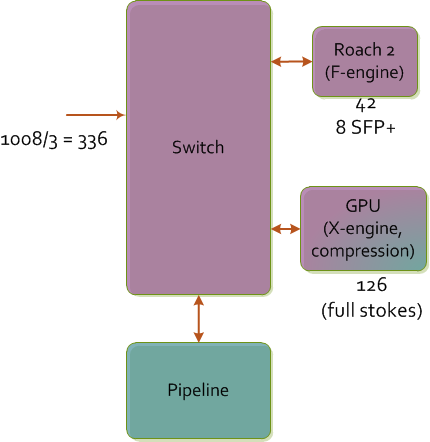
\includegraphics[width=0.55\textwidth]{plots/Digital.png}
\caption{Digital configuration.}
\label{fig:digital}
\end{figure}

The ROACH2 boards will serve as the F-engine for the correlator.  Each
has 8 bi-directional 10Gb SFP+ connectors.  Since at this point there are still
3 antennas per link, there are 1020/3 = 340 10GbE inputs.  
By dropping to 4b+4b real/imag for only positive frequencies, F engines have 1/2
the data output rate.  Hence each ROACH2 will need 5 ports reserved for inputing data
directly from the field, and 3 reserved for outputting data to the switch used for
the correlator corner-turn.  Hence 340/5 = 68 ROACH2 boards are required.
It is anticipated
that beyond the connectivity, 68 ROACH2 boards will have sufficient compute power
to host 15 F engines (a 32-antenna F-Engine design for ROACH2 has already been demonstrated).
F Engines will, in total, require 204 switch ports, for an aggregate output rate of 1632 Gbps.

GPUs will serve as X-engines in the correlator (and will also be used to compress data, as discussed 
in \S\ref{sec:data}). For HERA, we anticipate 2 Moore's Law doublings from currently deployed PAPER
technology (the Kepler 690 dual GPU card), allowing a 1024-element full-Stokes correlator to be implemented with
128 GPU boxes, each containing 1
CPU, 2 dual-GPUs, and 1 dual 10GbE NIC.
If full Stokes is not
needed (i.e. no U,V), the GPU system may possibly be reduced by a factor of 2.

The switch will need 204 + 256 = 460 ports.  If switches this large prove hard to find,
an alternate configuration, which may cost a bit more in ROACH2 hardware, could get the total number of switch
ports down to 170.

This correlator is anticipated to pull around 100 kW, of which $\sim$95 kW are the GPU boxes.  For an observing
season, this costs $\sim$\$40 kUSD.  Including cooling overhead, that cost rises to $\sim$\$80 kUSD.  Although this
is within a managable range, it may be worth examining lower-power alternatives.  

For 10-second integrations, the data output rate of the correlator will be 14 Gbps.  This is a managable
rate for recording to storage in the short term.  However, at 74 TB/day (and 13 PB per campaign), this
quickly becomes unwieldy, and a data management plan (did I just say that?) is required.

ISSUES: power consumption of GPUs is high.

\section{Data Management}

Given the sheer volume of data output from the correlator, a near-real-time processing system must
be in place to reduce data to a manageable volume.  A data compression scheme tailored to low-frequency
transit telescopes is described in Appendix A of \citet{parsons_et_al2013}.
As demonstrated on PAPER, this delay/fringe-rate compression scheme is nearly lossless from
the point of view of EoR emission locked to the celestial sphere.  Applying the full compression assuming
a maximum baseline length of 300m results in a 20x data reduction factor.  This reduces the data volume
from a campaign (180 days) to 610 TB.

Using benchmarks from
deployed PAPER data compression systems, and assuming a 10x speed-up per thread for implementing this
compression on GPUs (which preliminary results suggest is reasonable), we anticipate that 64 GPU boxes
will be sufficient to compress a 12-hour observation (74 TB) in 8 hours.  

Details of the processing/compression, leading to the use of the GPUs during the day to process.
This means a 500 TB drive would do the trick.

Data compression is somewhat computationally expensive.  However, scaling from currently known run-times
on a compute cluster (64$^2$/2 baselines in real time on 2 cores), assuming 2 Moore's Law doublings,
and assuming a factor of 10 scaling for computing on GPUs, we get that 205 single GPUs would be sufficient
to compress the data.  Fortunately, during the daytime, we have 256 dual GPUs available in the correlator.
The plan is to use these during the day to compress data.

If we want more flexibility in data analysis, we could temporarily store uncompressed data and then
LST bin.  This assumes no ionosphere correction, which hasn't been shown to work or be necessary.
We can debate this.

We should also have 2PB of tape storage for archiving.

\section{Infrastructure}
\label{sec:infra}

Need some.  A lot depends on piggybacking off of other facilities.  More to come here.

Operating power: 128 GPU boxes at 1kW, 68 ROACH2 at 200W + 10kW data = 152 kW.  Operating for 24 hrs (12
observing + 12 compression) for 300 days = 1.09e6 kWhr.  At \$0.10 per kWhr, this is \$110k.

\end{document}
